\documentclass[11pt]{article}
\usepackage[margin=25mm]{geometry}
\usepackage{amsmath,amssymb,booktabs,graphicx,xcolor}
\usepackage[colorlinks=true,linkcolor=blue,citecolor=blue,urlcolor=blue]{hyperref}
\newcommand{\pending}[1]{\textcolor{red!65!black}{#1}}
\graphicspath{{../research/4.temporal-consistency/report/exploration-r41-training-form/}{../research/4.temporal-consistency/report/exploration-r42-tlc/}{../research/4.temporal-consistency/report/exploration-r44-bounded-video/}{../research/4.temporal-consistency/report/exploration-r45-response-recursion/}}
\title{Temporally Stable Ultra-Compact Video Enhancement\\
\large Working manuscript: problem, protocol, and verified preliminary evidence}
\author{Internal research draft; authorship to be determined by the project team}
\date{Evidence snapshot: 13 November 2026}
\begin{document}
\maketitle
\begin{abstract}
Applying a compact image enhancer independently to video frames creates a
quality--stability problem under a tight computation budget. We formulate the
distinction between training-time temporal supervision and inference-time
history, establish strong same-weight classical references, and document
controlled evidence for adapting MobileIE. The completed experiments show that
restoring the original expanded training parameterization improves a matched
mixed-data baseline, while a fixed test-time local pooling conversion harms
both evaluated domains. A completed factorial study of the root nonlinearity
and a training-only temporal objective improves paired-real spatial quality
but fails all three registered temporal/deployment screens. Its spatial and
temporal effects must be separated. Matched learned-recursion controls also
show negligible benefit of an internal feature-energy cue over an RGB gate,
while exposing a quality--stability trade-off over fixed fusion weights.
Completed fixed-budget adaptations of a published 696-parameter enhancer,
a five-frame video denoiser, and a published deformation-consistency
objective extend reference coverage while retaining training-history,
convergence, and domain limitations. The fixed commutator adaptation
reduces paired-real temporal error at a substantial spatial and perceptual
cost; a fixed display-based metric further qualifies temporal-error gains.
Common convolution budgets are reported without inferring phone speed.
These findings do not establish a new video enhancement method.
This internal draft contains no independent
final-test claim or measured phone latency.
\end{abstract}

\paragraph{Draft status.}
\pending{This is a research manuscript under development, not a submission-ready
paper. The final method, verified novelty, independent low-light video
evaluation, and handset measurements remain incomplete.}
The numerical tables are generated from completed repository evidence.
Training progress, partial checkpoints, and loss curves are excluded.

\section{Problem and deployment constraints}
\label{sec:problem}
An image enhancer maps a low-light observation $x_t$ to an enhanced frame
$z_t=f_\theta(x_t)$. A video system must also preserve legitimate scene changes,
avoid noise-driven fluctuations, and fit its computation and memory budget.
Low parameter count alone does not establish any of these properties.
MobileIE~\cite{mobileie} provides a useful compact starting point. Our
12-channel low-light deployment instance has 4,075 parameters; \emph{4K parameters}
does not mean a video resolution of $4\mathrm{K}$.

We distinguish a stateless predictor from a stateful one:
\[
 z_t=f_\theta(x_t),\qquad
 (z_t,h_t)=F_\theta(x_t,h_{t-1}).
\]
A training objective may use neighbouring frames without introducing
$h_{t-1}$ at deployment. Conversely, a computation whose output changes for
two histories with the same current frame cannot generally be represented
exactly by a function of that current frame alone. Spatial convolution/BN
folding does not eliminate this information dependency.

Our evaluation therefore reports quality, temporal error, parameters,
convolution operations, online history, and measured pipeline latency as
separate quantities. A small parameter change can still introduce
full-resolution arithmetic or memory traffic. Inference motion estimation,
sampling, padding, and buffering belong to the deployed pipeline even when
they have no learned parameters. Server CPU measurements are not phone
measurements.

\subsection{The original nonlinear pathway}
The retained MobileIE backbone consists of a convolutional head, a second
feature block, channel/spatial gates, and an RGB readout~\cite{mobileie}.
Its feature self-transform (FST) has the form
\[
 q(u)=(w_1u)(w_2u)+b=a u^2+b,
\]
where $w_1,w_2$ are shared scalars and $b$ is channel-wise. Channel attention
uses global average pooling followed by a $12\!\times\!12$ pointwise map and
a sigmoid. The spatial gate depends on the channel-weighted feature maximum.
The learned enhancement mapping, global statistics, and local nonlinear
response can consequently interact.

For a scalar perturbation $\epsilon$, the identity
\[
 q(u+\epsilon)-q(u)=2au\epsilon+a\epsilon^2
\]
motivates examining noise sensitivity at the root operator. If the
perturbation has conditional mean zero, its conditional mean shift is
$a\,\mathbb E[\epsilon^2]$. This elementary identity is not a new
contribution. It neither proves that FST is the sole cause of video flicker
nor establishes an unbiased correction for features after nonlinear
convolutions, ISP processing, clipping, and quantization.

\subsection{Known mechanisms and the remaining research question}
Training-time reparameterization, channel multiplication, temporal
regularization, and classical motion-compensated fusion are established
tools. FastDVDnet~\cite{fastdvdnet}, for example, learns multiframe denoising
without an explicit flow estimator. TLC~\cite{tlc} addresses a different issue:
the spatial-statistic mismatch between patch training and whole-image
inference. Learnable safe rational activations also have clear
precedents~\cite{pau}.

The unresolved question is whether an independently justified video
adaptation can improve the quality--stability--cost trade-off over strong
matched controls in this extremely compact setting. Neither assembling these
known components nor obtaining a nonzero historical effect answers that
question. The current candidate remains an experiment until its controlled
results, external validity, and deployment costs support a defensible claim.

\section{Related mechanisms and the scope of differentiation}
\label{sec:related}
\paragraph{Temporal training with image inference.}
StableLLVE~\cite{stablellve} trains enhancement with synthetic motion and
temporal consistency while its released U-Net predicts one frame at a time.
Consequently, using temporal supervision without a deployed recurrent state
already has direct LLVE precedent. The released checkpoint is explicitly
trained on synthetic clean data and is qualified by its authors for noisy
inputs. Our earlier transfer experiment preserves this limitation; it does
not replace common-data training or establish a fair ranking against a
task-adapted compact model.

\paragraph{Explicit temporal information.}
FastDVDnet~\cite{fastdvdnet} and EMVD~\cite{emvd} illustrate two different
deployment choices: a multiframe window and recurrent fusion. EMVD combines
past observations recursively in a learned transform representation, then
denoises and restores detail. Its real-RAW setting differs from the present
RGB enhancement proxy. Neither a learned recurrent blend nor a small state
alone distinguishes a new method. Our classical recursive reference tests
the benefit of retained history, without claiming to reproduce EMVD.

\paragraph{Correspondence and decomposition.}
The 2026 VLLVE/VLLVE++ preprint~\cite{vllveplus} couples consistent
decomposition with deep cross-frame interaction. Its described inference
path uses a nearby reference frame; ablations also consider operation
without a reference. Correspondence refinement operates during training.
Removing that estimator alone does not remove the enhancement network's
reference dependence. The deployed information and operators must therefore
be stated explicitly. A training-only component does not establish
single-frame inference.

The present draft differentiates experimental questions and information
budgets, not an established novel method. A publishable contribution still
requires a specific mechanism with controlled gains, stronger external
validation, and measured deployment cost beyond these known ingredients.

\section{Candidate and controlled questions}
\label{sec:candidate}
\pending{The following candidate is being tested in the registered R44 study.
Its performance and independent contribution have not been established.}

\subsection{A constrained root nonlinearity}
We investigate the restricted rational response
\[
 q_\kappa(u)=\frac{a u^2}{1+\kappa(u/s)^2}+b,
 \qquad s>0,\quad \kappa\geq 0 .
\]
Each of the two FSTs receives one additional scalar $\kappa$. This is a
constrained member of the known rational-activation family~\cite{pau};
we do not claim the rational form, safe denominator, or learnable activation
as a new invention. At $\kappa=0$, the original response is recovered.
For positive $\kappa$,
\[
 q_\kappa'(u)=\frac{2au}{[1+\kappa(u/s)^2]^2},
 \qquad
 \sup_u|q_\kappa'(u)|
 =\frac{9|a|s}{8\sqrt{3\kappa}}.
\]
The maximum occurs at $|u|=s/\sqrt{3\kappa}$. This scalar derivative bound
does not establish a measured whole-network robustness or flicker bound;
it also diverges when $\kappa$ approaches zero.

The fixed scale $s$ is the pre-FST feature RMS from eight predetermined
training windows, computed separately for each layer and training seed.
Calibration uses only training inputs and discards the temporary BN states.
It fixes optimization units rather than selecting a scale on development
quality. The learned denominator remains in deployment. The resulting
predictor has 4,077 parameters, no temporal state in its raw path, and extra
pointwise arithmetic compared with the 4,075-parameter square predictor.
Only the spatial MBR convolutions and fixed-statistics BN are folded.

\subsection{Training-only target-change compensation}
Let $W_t$ gather the previous frame into current-frame coordinates and let
$m_t$ be its validity mask. The candidate temporal objective is
\[
 \mathcal L_{\rm time} =
 \frac{\sum_{t,p}m_t(p)
 \left\|[z_t-W_tz_{t-1}](p)
       -[y_t-W_ty_{t-1}](p)\right\|_2^2}
 {3\sum_{t,p}m_t(p)} .
\]
It is defined as zero when no points are valid. The frame reconstruction
term still updates in that case. Subtracting the target change allows
legitimate target motion or brightness change rather than assuming that
the desired video is constant. Correspondences are estimated from training
targets with the fixed half-resolution forward--backward estimator; they
are not motion truth. Both predicted frames receive gradients. Deployment
does not call this training correspondence estimator.

\subsection{Factorial control}
The fixed design crosses original square versus constrained rational FST
with frame MSE versus $\mathcal L_{\rm MSE}+0.25\mathcal L_{\rm time}$.
All four models start from the same completed expanded-training checkpoint
for each seed, with the same BN statistics. Adam is restarted for every
arm. Each final model inherits 4,000 updates and receives 4,000 additional
updates on the same prescribed windows. This controls for extra training,
the objective, and the structural change; equal image/update budgets do
not imply equal training FLOPs.

The primary structural screen compares the rational temporal model with
the square model under the same temporal objective. A separate stateless
deployment screen compares its raw output with both square controls'
recursive postprocessing. A third screen compares all models with
recursive postprocessing. A positive third screen cannot be reported as a
stateless or flow-free result. Each registered screen includes both domains,
both seeds, quality preservation, a temporal-error improvement requirement,
and a worst-condition quality bound.

\section{Experimental protocol and comparison scope}
\label{sec:protocol}
\subsection{Development data}
The current synthetic training pool contains 57 DAVIS training videos,
excluding the three development sources \emph{bear}, \emph{lucia}, and
\emph{walking}. The synthetic development pilot uses 64 frames per source,
at 480-pixel height, with two independently sampled noise conditions.
There are three source videos and six conditions, not six independent videos.
For a target RGB value $y$ in $[0,1]$, the degradation proxy is
\[
 v=0.35y^{2.2},\qquad
 x=Q_8\!\left(\operatorname{clip}
 \left[\operatorname{Poisson}(Pv)/P+\eta,0,1\right]\right),
 \quad \eta\sim\mathcal N(0,0.008^2),
\]
with $P\in\{20,80\}$. Here $Q_8$ denotes conversion to the eight-bit
observation. The present pilot adds no extra JPEG encoding, although the
source frames are JPEG images. This is a controlled synthetic proxy, not
a calibrated model of arbitrary RAW sensors or phone ISP video.

The fixed mixed-data study replaces half of each training batch with
native crops from 12 verified paired ND-filter video sources in the
project's OLiVES snapshot. Its four already-used paired-real development
sources are videos 15, 47, 91, and 121, each evaluated on 16 frames with a
$288\!\times\!512$ crop. Training and development source IDs are separated.
Consecutive registered frame indices are available; independent sensor
timestamps have not been verified. These daytime ND pairs must not be
presented as natural nighttime validation.

Three original phone clips have additionally been inspected without
synthetic degradation. They have no synchronized reference, so they support
behavioural examples rather than reference PSNR or a perceptual flicker
ranking. Independent final-test evaluation remains outstanding.

\subsection{Quality and temporal measurements}
Predictions are evaluated as floating-point RGB values after clipping to
$[0,255]$, before display rounding or video encoding. Sequence PSNR is the
mean of full-frame RGB frame PSNR values,
\[
 \operatorname{PSNR}_{\rm seq}
 =\frac1T\sum_t 10\log_{10}
 \frac{255^2}{\operatorname{MSE}_{\rm RGB}(z_t,y_t)}.
\]
RGB SSIM uses an $11\!\times\!11$ Gaussian window with standard deviation
1.5 and the valid region obtained by excluding five boundary pixels.
Edge MAE is the full-frame mean absolute error of horizontal and vertical
luminance Sobel gradients, with the fixed gradient normalization used by
the evaluation implementation.

For a fixed estimated reference flow and validity mask, temporal error is
\[
 E_{\rm temp}=\frac{1}{|\mathcal T|}\sum_{t\in\mathcal T}
 \frac{\sum_{p,c}m_t^{\rm ref}(p)
 \left|[z_t-W_t^{\rm ref}z_{t-1}]_c(p)
       -[y_t-W_t^{\rm ref}y_{t-1}]_c(p)\right|}
 {3\sum_p m_t^{\rm ref}(p)}.
\]
Here $\mathcal T$ contains frame pairs with nonempty valid masks. The
sequence summary first averages each valid frame pair, then averages
the available pairs. The reference mask excludes an
eight-pixel boundary. Reference flow is estimated from targets and held
fixed across compared methods; it is not ground-truth motion.
This metric is not a sufficient perceptual definition of flicker.
Evaluation uses fixed reference fields and absolute RGB error. Training
uses half-scale estimated fields, differentiable continuous bilinear
gathering, and squared error. The two are not numerically identical.

Domains and training seeds are reported separately before aggregation.
The present two-seed pilot does not establish statistical significance.
We retain per-condition failures alongside mean improvements.

\subsection{Strong same-weight references}
For each spatial anchor, let $r_t$ denote the raw prediction. The finite
reference uses the previous raw output, while recursive fusion uses the
previous fused output:
\[
 z_t^{\rm fin}=\tfrac12 r_t+\tfrac12 W_t r_{t-1},
 \qquad
 z_t^{\rm rec}=\tfrac12 r_t+\tfrac12 W_t z_{t-1}^{\rm rec}.
\]
The formulas apply only on accepted correspondences; invalid points and the
first frame use the current raw output. Both estimate motion from their own
adjacent raw predictions with the fixed half-resolution forward--backward
estimator. Recursive fusion therefore also keeps the previous raw output.
Neither reference requires a second enhancement CNN or a GT reset.

Published FastDVDnet weights~\cite{fastdvdnet} have been evaluated as
fixed denoiser transfer, not as a retrained low-light video method.
Its five-frame window uses two future frames. The documented pretraining
source includes the three current DAVIS development IDs, so that transfer
cannot establish unseen generalization. Same-domain retraining and broader
published LLVE comparisons remain necessary.

\subsection{Efficiency}
Convolution MACs, pointwise work, history storage, and full pipeline time
are distinct measurements. The original predictor has approximately
7.938 convolution GMAC at $1080\mathrm p$. This count omits non-convolution
work. Online history counts use actual tensor storage rather than only
logical channel slices. CPU timing is measured with two Torch threads and
one OpenCV thread, and its workload and reference weights are stated
explicitly. No handset latency is inferred from these measurements.

\section{Verified preliminary evidence}
\label{sec:evidence}
The following results come from completed development experiments. They
constrain method design; they are not evidence that the pending candidate
has succeeded. The source manifest and generated tables accompany this draft.

\subsection{A stronger training baseline}
\begin{table}[t]
\centering\small
\caption{Completed anchor evidence: two-seed means on custom synthetic and paired ND development data. Historical rows differ in training; only the two R41 raw forms are a matched FP32 parameterization comparison.}
\label{tab:anchors}
\begin{tabular}{lrrrr}
\toprule
Anchor/output & SYN PSNR & SYN $E_{\rm temp}$ & ND PSNR & ND $E_{\rm temp}$\\
\midrule
Dynamic synthetic (R34) & 26.234 & 10.505 & 23.453 & 3.166\\
Fixed mixed Slim (R40) & 25.134 & 11.363 & 24.861 & 3.628\\
Matched Slim FP32 (R41) & 25.131 & 11.362 & 24.861 & 3.627\\
Expanded FP32 (R41) & 26.186 & 10.007 & 25.847 & 3.630\\
Expanded + finite & 26.394 & 7.286 & 25.734 & 2.804\\
Expanded + recursive & 26.503 & 6.520 & 25.758 & 2.553\\
Earlier native training (R26) & -- & -- & 27.138 & 3.313\\
\bottomrule
\end{tabular}
\end{table}

Table~\ref{tab:anchors} separates historical anchors from the matched
training-form comparison. In the matched FP32 experiment, restoring MBR/BN
training improves synthetic raw PSNR over direct Slim fine-tuning by
0.968 and 1.142\,dB for the two seeds. The corresponding paired-real gains
are 0.171 and 1.799\,dB. Both deploy to the same 4,075-parameter spatial
class. Training parameterization is therefore a material baseline choice.
This is known spatial reparameterization, not a new video mechanism.

The expanded control uses 49,978 training parameters, including an inactive
frozen warm head; 47,239 parameters are optimized. It is a controlled
fine-tuning study, not a complete reproduction of the official warm-up,
loss, and long-schedule training. To preserve the pretrained numerical
starting function, the wide raw convolution executes its preserved and
additional output blocks separately. This retains its parameters and
mathematical operator but differs from the upstream single wide-kernel call.

The domain trade-off remains important. Expanded training approximately
recovers the synthetic quality of the dynamic-synthetic anchor while
improving its paired-real mapping. It still trails the earlier native
training reference in paired-real PSNR. Those historical training schemes
differ in several respects and do not isolate one causal factor.
No single online model is obtained by taking the best weight separately
for each domain.

\begin{figure}[t]
\centering
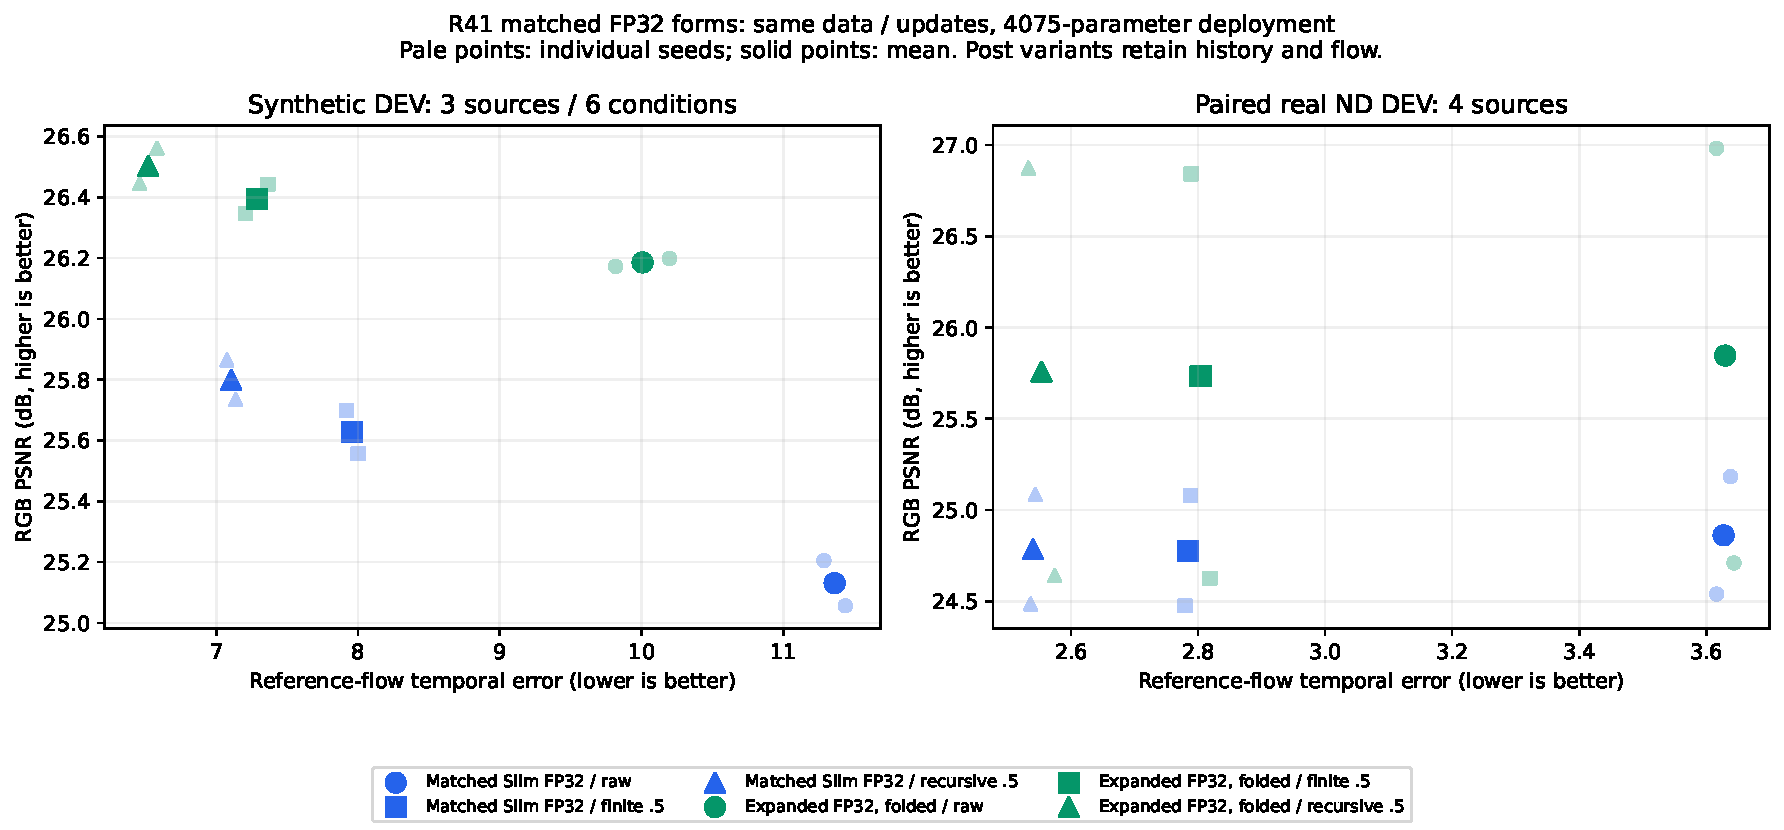
\includegraphics[width=\linewidth]{matched_forms.pdf}
\caption{Completed matched FP32 training-form comparison. Pale points retain
both individual seeds; solid points are their means. The real-domain spread
and the quality--temporal trade-off are visible. Postprocessed outputs use
motion and history; they are not stateless predictions.}
\label{fig:forms}
\end{figure}

Mean improvement does not imply reliable per-clip improvement. On paired-real
video 121, expanded seed 0 loses 2.606\,dB against its matched Slim control
and shows sky colour bias in the fixed-frame inspection. Its four-source
real mean is 24.710\,dB, versus 26.983\,dB for expanded seed 1. Raw
paired-real temporal error is not consistently reduced. All source/seed
pairs and all four metrics remain part of the record.

\subsection{Classical recursion is a necessary reference}
\begin{table}[t]
\centering\small
\caption{Classical references on the same R34 weights. Quality uses the full synthetic pilot. Resident CPU timing uses only the first 16 bear/P20 frames at $480\times854$, two Torch threads and one OpenCV thread. Ranges are run-average extrema, not confidence intervals or phone timings.}
\label{tab:classical}
\begin{tabular}{lrrrr}
\toprule
Output & PSNR & $E_{\rm temp}$ & History MiB & CPU ms/frame [range]\\
\midrule
Raw & 26.234 & 10.505 & 0.000 & 100.9 [80.9, 106.5]\\
Finite .5 & 26.466 & 7.543 & 4.691 & 184.1 [168.1, 188.5]\\
Recursive .5 & 26.610 & 6.735 & 9.382 & 186.5 [179.6, 192.5]\\
\bottomrule
\end{tabular}
\end{table}

On the same strong dynamic-synthetic anchor, recursive fusion improves
the finite reference's quality and temporal error
(Table~\ref{tab:classical}). Its persistent fused output is a meaningful
information advantage, not a negligible implementation detail. The
recursive reference cannot be replaced by a weaker two-frame average
when judging a proposed temporal model.

The measured CPU ranges overlap, so the small difference between the finite
and recursive medians is not established as a significant speed difference.
These timings concern the stated R34 weights and workload; they are not
measurements of the later expanded anchor or the pending rational model.
The extra stored RGB history and motion work remain part of deployment.

\subsection{Fixed local statistics do not rescue this anchor}
\begin{table}[t]
\centering\small
\caption{Fixed known TLC192 versus the same R41 expanded weights. No retraining or window search.}
\label{tab:tlc}
\begin{tabular}{llrr}
\toprule
Domain & Seed & Raw $\Delta$PSNR & Raw temporal ratio\\
\midrule
Synthetic & 0 & -0.305 & 1.0114\\
Synthetic & 1 & -0.415 & 1.0082\\
Paired ND & 0 & -2.312 & 1.0416\\
Paired ND & 1 & -2.343 & 1.0268\\
\bottomrule
\end{tabular}
\end{table}

The fixed TLC~\cite{tlc} control replaces only the channel-pooling node
with exact local averaging at a window of 192 pixels. Both development
domains and both seeds lose raw PSNR; the paired-real temporal ratios also
exceed the registered 1.02 upper bound (Table~\ref{tab:tlc}).
Across the 20 raw seed--condition pairs, five PSNR deltas are positive,
but all eight paired-real deltas are negative. The worst paired-real
condition loses 3.716\,dB.

The fixed instance and its local window search are stopped. This result
does not prove that all local aggregation or global-statistic adaptations
are ineffective. It also does not justify a speed claim: localizing the
channel map adds approximately 0.299 convolution GMAC at $1080\mathrm p$,
with prefix sums and memory traffic additional to that count.

\subsection{Pending candidate results}
\pending{The R44 factorial is still running at this manuscript snapshot.
Its raw, finite, recursive, per-condition, and per-seed final results must
be inserted only after both complete budgets and deployment-export gates
finish normally. No current loss curve or intermediate checkpoint supplies
this missing evidence.}

\subsection{Internal cues versus generic learned recursion}
\label{sec:r45}
\begin{table}[t]
\centering\small
\caption{Complete R45 comparison on the same frozen square-MSE base. Both-seed means; all fixed alpha points retained. All outputs except raw use motion and RGB history. Parameters omit unlearned motion work; no phone or pipeline cost is inferred.}
\label{tab:r45}
\begin{tabular}{lrrrrr}
\toprule
Output & Params & SYN PSNR & SYN $E_{\rm temp}$ & ND PSNR & ND $E_{\rm temp}$\\
\midrule
Raw & 4075 & 26.466 & 9.900 & 27.128 & 3.653\\
Fixed $\alpha=.1$ & 4075 & 26.733 & 8.922 & 27.188 & 3.316\\
Fixed $\alpha=.25$ & 4075 & 26.932 & 7.768 & 27.217 & 2.940\\
Fixed $\alpha=.5$ & 4075 & 26.707 & 6.470 & 27.108 & 2.570\\
Fixed $\alpha=.75$ & 4075 & 25.556 & 5.860 & 26.721 & 2.475\\
Fixed $\alpha=.9$ & 4075 & 23.833 & 5.936 & 26.147 & 2.575\\
Learned global & 4076 & 26.922 & 7.893 & 27.218 & 2.979\\
RGB gate & 4116 & 27.112 & 7.141 & 27.234 & 2.734\\
Internal cue & 4116 & 27.116 & 7.122 & 27.232 & 2.741\\
\bottomrule
\end{tabular}
\end{table}

The next fixed experiment asks whether the compact network's internal
response provides useful information beyond RGB for controlling history.
Learned fusion has established precedent~\cite{emvd}; it is a reference
mechanism here. The same square-MSE spatial checkpoint is frozen for each
seed. A global scalar, a 41-parameter RGB gate, and a matched 41-parameter
internal-cue gate each receive 4,000 updates using common four-frame windows
and MSE. Own-raw motion, acceptance masks, and recursion are shared.
All start from the classical $\alpha=.5$ function.

The internal inputs are two maps,
\[
 c(u)=\log\!\left(1+2|w_1w_2|\operatorname{RMS}_{C}(u)\right),
\]
read before the head and body FSTs in the same unchanged spatial forward
pass. For a square FST, derivative RMS is simply a fixed rescaling of
feature RMS. These maps are not an independent uncertainty theory or a
calibrated output variance. The RGB gate replaces those two inputs with
RGB chroma-deviation summaries while retaining the same capacity and six
common RGB/motion summaries.

Both complete budgets and frozen-backbone checks pass. Final CPU evaluation
finishes 180 rows and 20 CNN sequence calls; the latter capture cues and
replay the earlier raw predictions with maximum discrepancy zero.
Table~\ref{tab:r45} reports all five prescribed fixed weights and all learned
controls. Neither domain nor seed is selected after evaluation.

The internal-cue result is nearly indistinguishable from the RGB control.
Synthetic seed PSNR gains are only 0.0044 and 0.0027\,dB; paired-real
changes are $-0.0017$ and $-0.0024$\,dB. Temporal ratios versus RGB are
0.9969--0.9978 on synthetic data and 1.0025--1.0031 on paired-real data.
The registered independent-cue screen fails. Against fixed $\alpha=.5$,
quality improves but temporal error increases by about 6--11\%; that is
not joint superiority under the registered criterion.

Generic learning remains a useful control. Both pixelwise gates choose
accepted-pixel mean history weights around 0.34--0.36, compared with
0.228--0.236 for the learned global scalar. They are not jointly dominated
by any of the five sampled fixed-weight points. This does not establish
superiority over the continuous weight curve or an internal-cue contribution.
Increasing fixed history weight to 0.9 lowers PSNR substantially and can
also worsen temporal error. Motion error, resampling, occlusion, and bias
remain possible causes; this experiment does not isolate one of them.

The feature-RMS controller's local architecture/input/objective/optimizer
search is stopped. All controls are retained, and no candidate-specific
pipeline or handset cost is inferred from this shared-computation quality
experiment.

\begin{figure}[t]
\centering
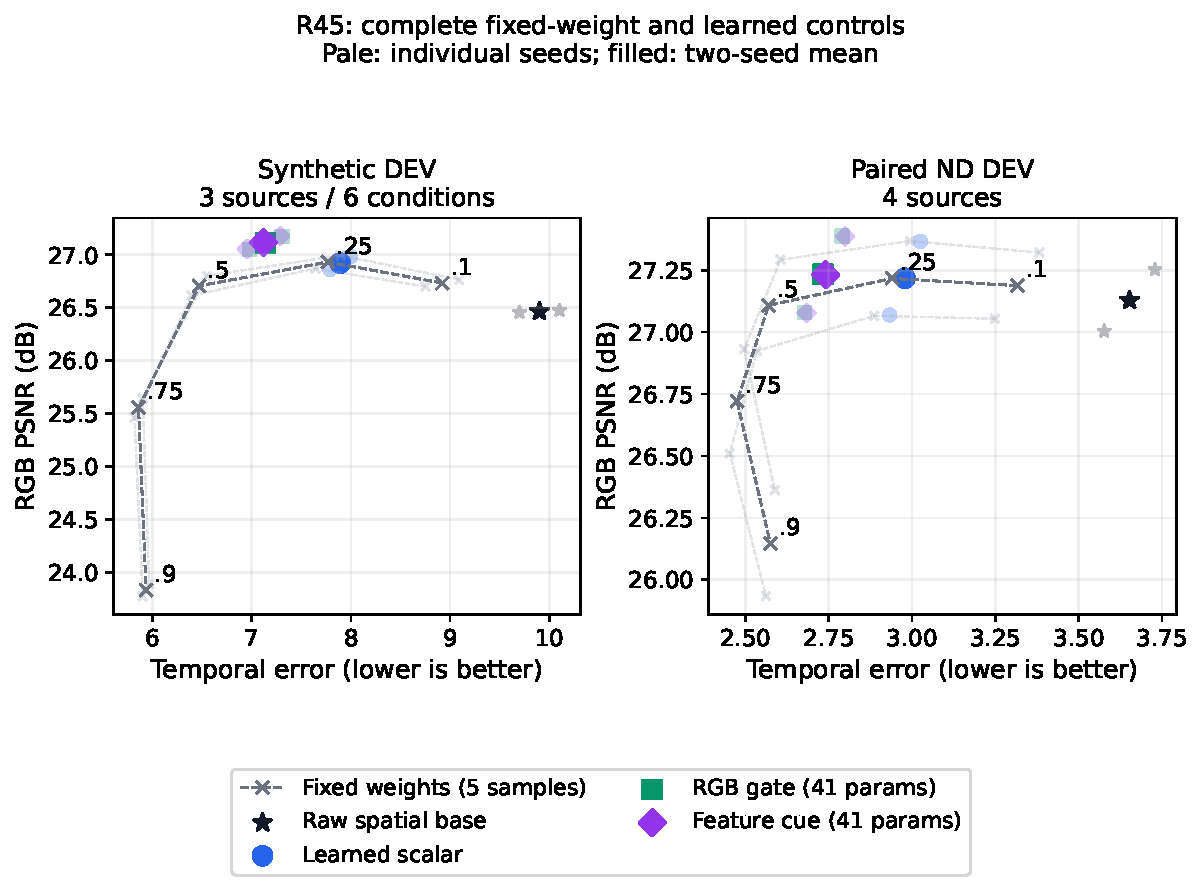
\includegraphics[width=\linewidth]{frontier.pdf}
\caption{Complete R45 fixed-weight sample and learned controls. Pale traces
and points retain both seeds. The RGB and internal-cue gates nearly overlap;
their generic trade-off cannot be credited to an independent internal-cue
mechanism. These are development results, not latency or final-test points.}
\label{fig:r45}
\end{figure}

\section{Published-loss adaptation, perception and reference cost}
\label{sec:video-evidence}
\paragraph{A controlled published-loss reference.}
We adapt the official 4,316,259-parameter StableLLVE U-Net
and deformation-consistency loss form~\cite{stablellve} to the fixed mixed
task. Both arms use the same public clean initialization, source windows,
BGR ordering and 8,000 updates per seed. The spatial arm minimizes L1;
the second adds $20\lVert F(Wx)-WF(x)\rVert_1$, retaining both prediction
paths' gradients. Here $W$ uses training-GT motion as a deformation field
applied to the same noisy source image. It does not create a separately
noised adjacent observation. Compared with the paper, this changes CMP
motion synthesis, crop size, initialization and training schedule. The
original warp coordinate convention and CUDA backward nondeterminism
are disclosed. This is a fixed-budget task adaptation, not a full
reproduction, a convergence claim or a new method.

\begin{table}[t]
\centering\scriptsize\setlength{\tabcolsep}{4pt}
\caption{Complete StableLLVE network/loss task adaptation. Every arm starts from the same public clean checkpoint and receives 8,000 updates per seed. The official L1 and weight-20 commutator form are retained, but training flow source, crop, initialization and schedule differ from the paper. Raw has no history/future input; rec. adds classical motion/history. JOD uses the fixed nominal display conditions in Table~\ref{tab:perceptual}. This is neither a new method nor a full-paper reproduction.}
\label{tab:stablellve-adapted}
\begin{tabular}{llrrrrrr}
\toprule
Loss/output & Seed & SYN PSNR & SYN $E_{\rm temp}$ & SYN JOD & ND PSNR & ND $E_{\rm temp}$ & ND JOD\\
\midrule
L1 raw & 0 & 28.087 & 7.619 & 7.657 & 28.732 & 3.235 & 8.432\\
L1 raw & 1 & 28.033 & 7.622 & 7.639 & 28.420 & 3.697 & 8.208\\
L1 + rec. & 0 & 27.590 & 5.493 & 7.632 & 28.582 & 2.437 & 8.430\\
L1 + rec. & 1 & 27.547 & 5.497 & 7.613 & 28.578 & 2.741 & 8.247\\
L1 + commute20 raw & 0 & 25.368 & 7.743 & 6.992 & 25.853 & 2.905 & 7.765\\
L1 + commute20 raw & 1 & 25.246 & 7.875 & 6.972 & 25.828 & 2.905 & 7.676\\
L1 + commute20 + rec. & 0 & 25.204 & 5.789 & 6.912 & 25.632 & 2.353 & 7.651\\
L1 + commute20 + rec. & 1 & 25.147 & 5.859 & 6.895 & 25.579 & 2.344 & 7.562\\
\bottomrule
\end{tabular}
\end{table}

Table~\ref{tab:stablellve-adapted} contains only the four final 8,000-update
models. Relative to its same-network spatial control, the commutator arm
loses 2.59--2.88\,dB raw PSNR and 0.53--0.67 predicted JOD across domains
and seeds. SYN temporal error increases by 1.63--3.32\%; paired-real
error decreases by 10.19--21.44\%, with lower spatial and perceptual
quality. Applying the same recursive reference does not remove this
trade-off. This fixed loss setting is stopped without a local weight,
geometry, learning-rate, crop or training-length search. It does not
invalidate the original paper or all equivariance objectives.

The L1 control is a useful stronger spatial reference: SYN raw PSNR is
28.03--28.09\,dB, and its recursive temporal error is 5.49--5.50 versus
6.39--6.55 for the MobileIE recursive reference. However, its raw temporal
error remains worse than that strong recursive reference. On paired-real
seed 1, even its recursive error is 2.74 versus MobileIE's 2.53. Capacity,
loss, pretraining and compute differ together; their separate effects
cannot be inferred from this comparison. All 20 preassigned static
contacts were inspected, including native center crops. These contacts
are not full-video playback or human flicker judgments.

\paragraph{Matching the spatial objective does not close the gap.}
\begin{table}[t]
\centering\scriptsize\setlength{\tabcolsep}{4pt}
\caption{Matched original MobileIE objective settings, final 8,000 updates only. Both objectives use the same source-window schedule, expanded training parameterization and two-stage Adam budget; L1/MSE gradient scale interacts with clipping. Every row deploys 4,075 parameters. Rec. adds the same classical motion/history reference. SYN comprises three source videos under two noise conditions; ND comprises four reused development clips. JOD uses the fixed assumptions in Table~\ref{tab:perceptual}. No objective search, human study, handset or independent final-test claim.}
\label{tab:matched-objective}
\begin{tabular}{llrrrrrr}
\toprule
Objective/output & Seed & SYN PSNR & SYN $E_{\rm temp}$ & SYN JOD & ND PSNR & ND $E_{\rm temp}$ & ND JOD\\
\midrule
MSE raw & 0 & 26.475 & 10.102 & 7.040 & 27.252 & 3.729 & 8.414\\
MSE raw & 1 & 26.456 & 9.699 & 7.111 & 27.004 & 3.577 & 8.552\\
MSE + rec. & 0 & 26.800 & 6.546 & 7.424 & 27.292 & 2.605 & 8.373\\
MSE + rec. & 1 & 26.613 & 6.393 & 7.409 & 26.923 & 2.534 & 8.512\\
L1 raw & 0 & 26.301 & 9.836 & 7.083 & 26.227 & 3.685 & 7.936\\
L1 raw & 1 & 26.492 & 9.351 & 7.104 & 26.633 & 3.474 & 8.428\\
L1 + rec. & 0 & 26.545 & 6.443 & 7.408 & 26.189 & 2.600 & 7.892\\
L1 + rec. & 1 & 26.531 & 6.279 & 7.354 & 26.566 & 2.512 & 8.382\\
\bottomrule
\end{tabular}
\end{table}

We separately train original MobileIE with spatial L1 under the same
source-window schedule and two-stage 8,000-update budget as its existing
MSE reference (Table~\ref{tab:matched-objective}). The original expanded
training graph and initialization are retained; both deploy the same
4,075-parameter graph. The comparison concerns the full objective setting:
different gradient scales interact with the shared gradient-clipping rule.
Only the preassigned final weights are evaluated.

L1 does not give a consistent joint improvement. Raw temporal error falls
by 1.18--3.59\%, while paired-real raw PSNR falls by 0.37--1.03\,dB and
predicted JOD by 0.12--0.48. Recursive temporal error falls by only
0.22--1.80\%, again with quality costs. SYN seed 1 raw gains just
0.036\,dB while predicted JOD decreases slightly. This fixed reference
is retained without an objective-mixture, learning-rate or seed search.
All 20 prescribed contacts were inspected, without full-video playback
or a human temporal study.

With both spatial references trained using L1, the U-Net still has
1.54--1.79\,dB higher SYN raw PSNR and 1.79--2.51\,dB higher paired-real
raw PSNR. Thus the objective difference alone does not account for the
observed gap, but architecture, capacity, pretraining and optimization
remain coupled. This comparison does not identify capacity as the cause
or establish a new temporal method.

\paragraph{Perceptual predictions qualify the temporal proxy.}
\begin{table}[t]
\centering\small
\caption{Full-reference ColorVideoVDP v0.5.7 predictions for the existing references, with both adapted seeds. The original StableLLVE clean checkpoint has zero project updates and no training seed. Nominal 30\,fps, original-sized SDR arrays, standard FHD display, 37.84 pixels/degree, 200\,cd/m$^2$ peak and replicate temporal padding are assumed. These JOD predictions are not measured handset viewing, capture timing, human MOS or a separately calibrated flicker score.}
\label{tab:perceptual}
\begin{tabular}{llrr}
\toprule
Reference/output & Seed & SYN JOD & ND JOD\\
\midrule
MobileIE raw & 0 & 7.040 & 8.414\\
MobileIE raw & 1 & 7.111 & 8.552\\
MobileIE + rec. & 0 & 7.424 & 8.373\\
MobileIE + rec. & 1 & 7.409 & 8.512\\
Nano raw & 0 & 6.742 & 8.169\\
Nano raw & 1 & 6.872 & 8.141\\
Nano + rec. & 0 & 7.118 & 8.114\\
Nano + rec. & 1 & 7.178 & 8.080\\
FastDVDnet window & 0 & 7.432 & 7.680\\
FastDVDnet window & 1 & 6.304 & 7.257\\
StableLLVE clean raw & -- & 6.262 & 6.802\\
StableLLVE clean + rec. & -- & 6.266 & 6.632\\
\bottomrule
\end{tabular}
\end{table}

We evaluate ColorVideoVDP~\cite{colorvideovdp} on the complete cached
sequences with one fixed display configuration
(Table~\ref{tab:perceptual}). The combined collection has 220
sequence-condition rows and 9,856 comparison frames, reusing 448 input
observations; ten GT identity controls return exactly 10. These are
repeated conditions, not independent video samples. In particular, the
six SYN conditions are three source videos under two noise conditions.
No enhancement network is rerun to obtain these scores.

For MobileIE on SYN, recursion improves predicted JOD by 0.30--0.38
alongside lower temporal error. On paired-real, the mean JOD changes
are about $-0.04$ despite roughly 29--30\% lower temporal error. The
negative change is concentrated in video 15, while the other three
sources have positive changes for both seeds. These small means are
not evidence of statistically significant or human-perceived degradation.
The spatially adapted U-Net also shows that lower temporal error need
not improve JOD: on SYN its recursive JOD is about 0.026 below raw.
Predicted perceptual quality, spatial fidelity and the temporal residual
therefore need joint reporting. A dedicated human temporal study remains
necessary; no display-condition grid is used to select favorable scores.

\paragraph{Efficiency remains a separate empirical requirement.}
\begin{table}[t]
\centering\small
\caption{Reference deployment conditions at $1080\times1920$, batch one, per output frame. Conv GMAC counts only executed Conv2d multiply--accumulates; it omits bias, resizing, priors, pooling, activation, motion, warping and memory work. FastDVDnet uses the original uncached three first-stage and one second-stage calls. Rec. additionally retains two FP32 RGB frames plus motion/workspace; raw spatial networks have no temporal state. Identical StableLLVE graphs serve its public and adapted weights. No row is a measured handset latency or complete pipeline FLOP claim.}
\label{tab:reference-budget}
\begin{tabular}{lrrrrl}
\toprule
Network/output & Params & Conv GMAC & Future & Flow & Handset ms\\
\midrule
MobileIE raw & 4075 & 7.938 & 0 & no & --\\
MobileIE + rec. & 4075 & 7.938 & 0 & yes & --\\
Nano raw & 696 & 1.313 & 0 & no & --\\
Nano + rec. & 696 & 1.313 & 0 & yes & --\\
FastDVDnet window & 2479096 & 1319.208 & 2 & no & --\\
StableLLVE raw & 4316259 & 317.240 & 0 & no & --\\
StableLLVE + rec. & 4316259 & 317.240 & 0 & yes & --\\
\bottomrule
\end{tabular}
\end{table}

The common Conv2d convention in Table~\ref{tab:reference-budget} gives
317.24\,GMAC for StableLLVE versus 7.94 for MobileIE at 1080p. This
approximately forty-fold convolution-budget difference cannot be
translated into a phone-latency ratio. The count excludes motion,
warping, point operations and memory traffic, and the largest individual
convolution output is not peak memory. Neither the 4,075-parameter
starting point nor zero added inference cost is an imposed hard limit.
A defensible deployment claim requires actual full-pipeline phone
measurements for a candidate that first demonstrates joint quality and
stability gains. No such new candidate is established by these references.

\section{Fixed classical block-matching reference}
\label{sec:classical-reference}
We evaluate the original numerical core and default initialization of the
IPOL VBM3D implementation~\cite{vbm3d_ipol} through an array interface,
without changing its filtering or color-transform code. The spatial-only
control disables temporal search ($N_f=0$); the video control retains
default temporal search ($N_f=4$) on each full offline clip. Both receive
one blind noise estimate from the first low-light frame: the median over
RGB channels of centered Haar-HH MAD estimates, divided by $0.67448975$
in the implementation's 8-bit amplitude units. No clean frame or known
degradation parameter enters this estimate. One filtered input is reused
by the two frozen 8,000-update MobileIE seeds. The same optional
own-output motion-compensated recursive reference is then applied.

\begin{table}[t]
\centering\scriptsize\setlength{\tabcolsep}{4pt}
\caption{Fixed original-core block-matching prefilters followed by the same frozen MobileIE weights. S-only disables temporal search in the VBM3D implementation; it is not an optimized BM3D reproduction. V-default uses the original video search on a full offline clip. A single blind first-frame noise estimate is shared by both modes. Rec. adds the same own-output motion/history reference. These reused development results and fixed-display JOD predictions do not establish calibrated noise, human judgments or a new method.}
\label{tab:classical-block}
\begin{tabular}{llrrrrrr}
\toprule
Prefilter/output & Seed & SYN PSNR & SYN $E_{\rm temp}$ & SYN JOD & ND PSNR & ND $E_{\rm temp}$ & ND JOD\\
\midrule
None raw & 0 & 26.475 & 10.102 & 7.040 & 27.252 & 3.729 & 8.414\\
None raw & 1 & 26.456 & 9.699 & 7.111 & 27.004 & 3.577 & 8.552\\
None + rec. & 0 & 26.800 & 6.546 & 7.424 & 27.292 & 2.605 & 8.373\\
None + rec. & 1 & 26.613 & 6.393 & 7.409 & 26.923 & 2.534 & 8.512\\
S-only raw & 0 & 24.351 & 8.142 & 6.917 & 26.689 & 3.525 & 8.383\\
S-only raw & 1 & 24.204 & 7.778 & 6.959 & 26.479 & 3.380 & 8.530\\
S-only + rec. & 0 & 24.278 & 5.772 & 6.931 & 26.725 & 2.540 & 8.328\\
S-only + rec. & 1 & 24.043 & 5.646 & 6.923 & 26.411 & 2.474 & 8.475\\
V-default raw & 0 & 23.978 & 7.554 & 6.781 & 26.605 & 3.466 & 8.380\\
V-default raw & 1 & 23.807 & 7.233 & 6.816 & 26.394 & 3.327 & 8.527\\
V-default + rec. & 0 & 23.878 & 5.707 & 6.749 & 26.641 & 2.522 & 8.324\\
V-default + rec. & 1 & 23.637 & 5.599 & 6.735 & 26.328 & 2.459 & 8.471\\
\bottomrule
\end{tabular}
\end{table}


The two controls are deliberately limited: spatial-only VBM3D is not an
optimized BM3D reproduction, and a full-clip video call is not a causal
deployment. Its search radius alone does not certify an end-to-end
future-wait bound across the filtering stages. An AWGN-oriented blind
scalar is also not calibrated to the Poisson, clipping and quantization
pipeline, or to a real camera ISP. Enhancement weights are held fixed,
so changes in their input distribution remain another possible cause;
these causes have not been isolated.

All 16 domain--seed--filter--output means lower the temporal-error proxy
but also lower PSNR and predicted JOD relative to the matching unfiltered
enhancer output. On SYN, raw PSNR decreases by $2.124$--$2.649$\,dB and
recursive PSNR by $2.522$--$2.976$\,dB. On paired-real ND, PSNR decreases
by $0.513$--$0.651$\,dB and predicted JOD by $0.022$--$0.050$.
The latter small metric differences are not human preference or a
significance claim. All 20 registered first/middle/last-frame contacts
were actually inspected: grain reduction coexists with softer fur,
stone and grass details; filtered recursive walking outputs show
building-edge distortions. These sparse contacts neither replace full
video inspection nor establish a causal mechanism or subjective score.

\begin{table}[t]
\centering\small
\caption{Descriptive CPU2 complete input-filter stages, including array I/O, in seconds per frame. Medians are over the registered sequence conditions; SYN has three source videos under two noise conditions. The same filtered input is reused across two enhancement seeds, so filtering is counted once. Shared-server timings have no isolated repeated latency trial and are not handset speed or an end-to-end future-wait bound.}
\label{tab:classical-cost}
\begin{tabular}{llrrr}
\toprule
Domain/size & Mode & Conditions & Median s/frame & Range\\
\midrule
SYN $480\times854$ & S-only & 6 & 1.824 & 1.816--1.907\\
SYN $480\times854$ & V-default & 6 & 5.249 & 5.220--5.280\\
ND $288\times512$ & S-only & 4 & 0.677 & 0.658--0.695\\
ND $288\times512$ & V-default & 4 & 1.774 & 1.739--1.776\\
\bottomrule
\end{tabular}
\end{table}


Table~\ref{tab:classical-cost} retains descriptive complete filtering
costs, including array I/O, from the registered shared-server CPU run
with two CPU threads. Filtering is counted once across enhancement
seeds. The measurements are not isolated repeated latency trials,
handset measurements, full operation counts, or evidence for a 4K
extrapolation. This fixed reference yields no robust joint quality and
stability improvement. We retain it without searching noise estimates,
windows, strengths or additional seeds, and keep the stronger
unfiltered MobileIE recursive reference. This result neither rules out
traditional denoising in general nor establishes a new method.

\section{Limitations and requirements for a complete paper}
The present development pilot is small and repeatedly used. Synthetic
noise, three DAVIS sources, and four paired daytime ND crops cannot
establish general low-light video performance. The inspected phone clips
show clipping and colour failures without synchronized ground truth.
They do not replace a reference-based nighttime benchmark or a perceptual
temporal study. Two training seeds expose variability but do not resolve it.

Motion-compensated target-residual error helps separate desired changes
from unwanted differences, but its estimated reference flow can fail and
its valid mask excludes difficult regions. Spatial quality, per-condition
failures, scene-change behaviour, and visual examples must accompany it.
Lower temporal error alone is insufficient: an inappropriate enhancement
mapping may also look numerically stable.

Published-weight transfers and fixed-budget task adaptations retain
input-domain, convergence, training-compute and pretraining-overlap
limitations. The completed Nano, source-context FastDVDnet and StableLLVE adaptations
improve reference coverage but are not full standard LLVE reproductions.
The fixed-display ColorVideoVDP predictions do not replace a human
perceptual study, measured capture timing or handset viewing conditions.
A conference comparison still requires appropriate published temporal
enhancement methods under a documented common setting.
The fixed classical references are strong controls, not full reproductions
of all established video denoisers.

No candidate in this snapshot has a verified independent contribution or
measured handset trade-off. A complete paper must establish the final method,
explain its difference from relevant prior art, pass controlled
structural/objective comparisons, measure
the complete inference pipeline and state on a phone, and evaluate frozen
decisions on genuinely independent data. The completed candidate's failure
must guide a distinct hypothesis, with the registered local search stopped.
Its spatial signal cannot be rewritten as temporal success. These
requirements preserve the original research objective;
the present manuscript is only the reusable foundation.


\clearpage
\bibliographystyle{plain}
\begingroup
\small
\bibliography{references}
\endgroup
\end{document}
